%\section{Applying cuts to the same flavour channel}
\section{First view}

A common practice in SUSY dilepton analyses is to divide events into same flavour (SF) and different flavour (DF) varieties. SF thus includes events with pairs of only electrons or only muons in their final states, and DF refers to the events that decay into an electron-muon pair. In this analysis this convention will be followed.

The preliminary cuts on the pair of electrons were $\mathbf{p}_{\text{T},e_1}>$ 25 GeV and $\mathbf{p}_{\text{T},e_2}>$ 20 GeV, where $e_1$ refers to the leading lepton with the largest momentum and $e_2$ to the second one.  For a muon pair the following requirements were imposed: leading muon $\mathbf{p}_{\text{T},\mu_1}>$ 25 GeV, second muon $\mathbf{p}_{\text{T},\mu_2}>$ 10 GeV, and the invariant mass $m_{\mu \mu}>$ 20 GeV. These cuts were motivated by the trigger efficiency for offline lepton candidates' identification (see Fig. \ref{fig:eltrig} and \ref{fig:mutrig} in the appendix \ref{app:triggers}).

First, histograms showing the entirety of the 2015 data, MC background and signal simulations were plotted. Fig. \ref{fig:SF_total_mll} shows the distribution of the \dileptonmass \, in the SF channel. The largest background contributions come from $Z$+jets, diboson, and $t\bar{t}$ processes. 
The pronounced peak in the SF dilepton invariant mass distribution is in the 80-100 GeV bin due to the contribution from the $Z$+jets component. This background can be suppressed by introducing $m_Z$-veto which cuts out all events within 10 GeV from the mass of the $Z$ boson (91.2 GeV). However, after this cut, the distribution will still retain events from the off mass-shell decays of the $Z$ boson. 

The histogram for DF channel (Fig. \ref{fig:DF_total_mll}) shows that there is a much smaller contribution from $Z$+jets component in this channel compared to the SF one. Thus $m_Z$ veto here can be avoided. The diboson and $t\bar{t}$ processes, however, prevail in this channel as well. 

\begin{figure}[!th]	   
	\begin{subfigure}[t]{0.5\textwidth}
		\subcaption{} 
		\label{fig:SF_total_mll}
        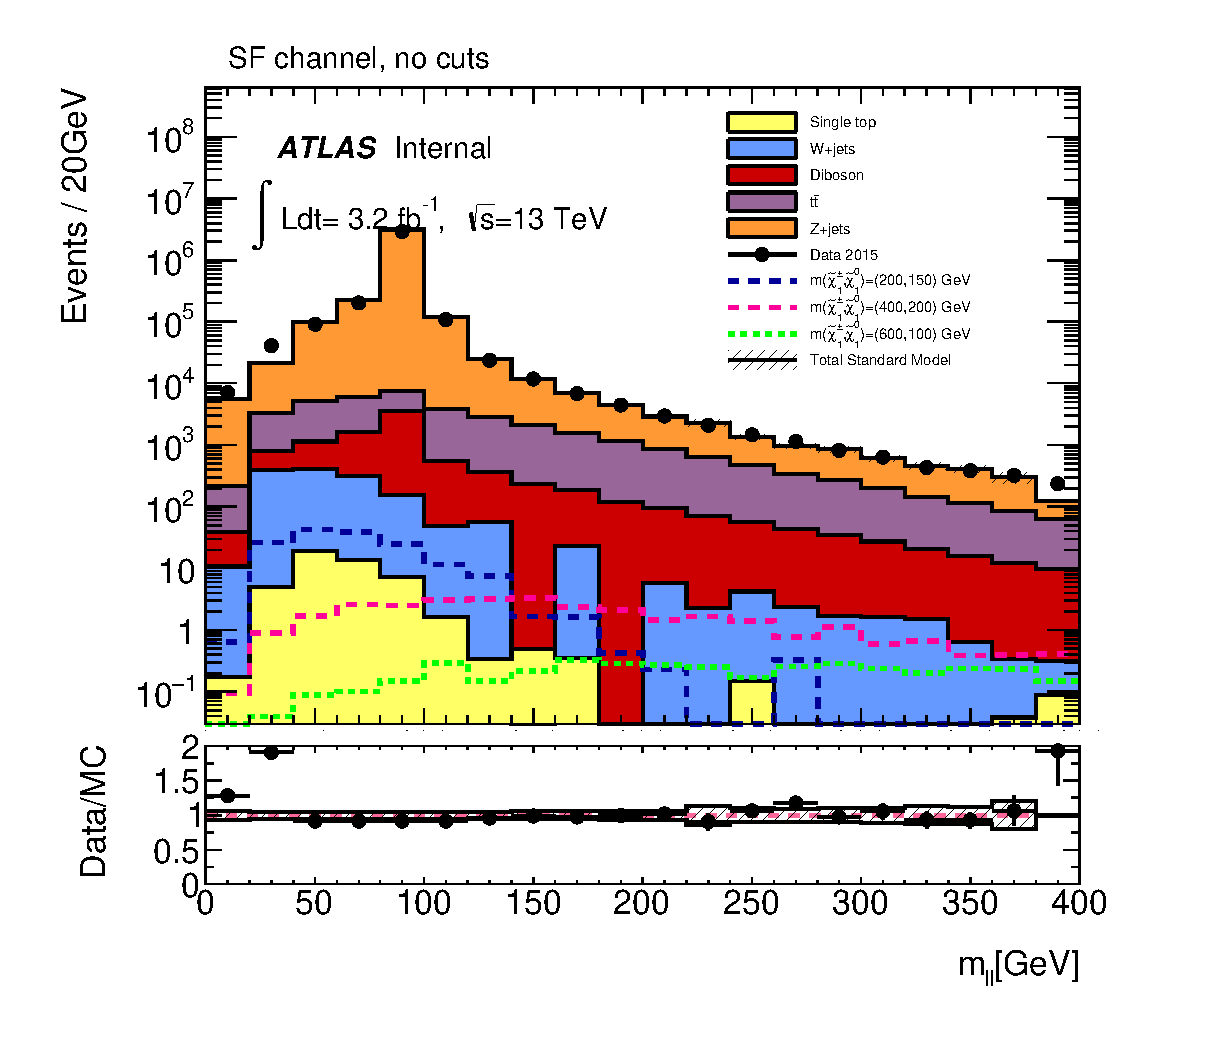
\includegraphics[scale=0.35]{Chap4/SF_DileptonMll_13TeV_total_signal} 
        \end{subfigure} 
     \begin{subfigure}[t]{0.5\textwidth}
     \subcaption{}
     	\label{fig:DF_total_mll}
        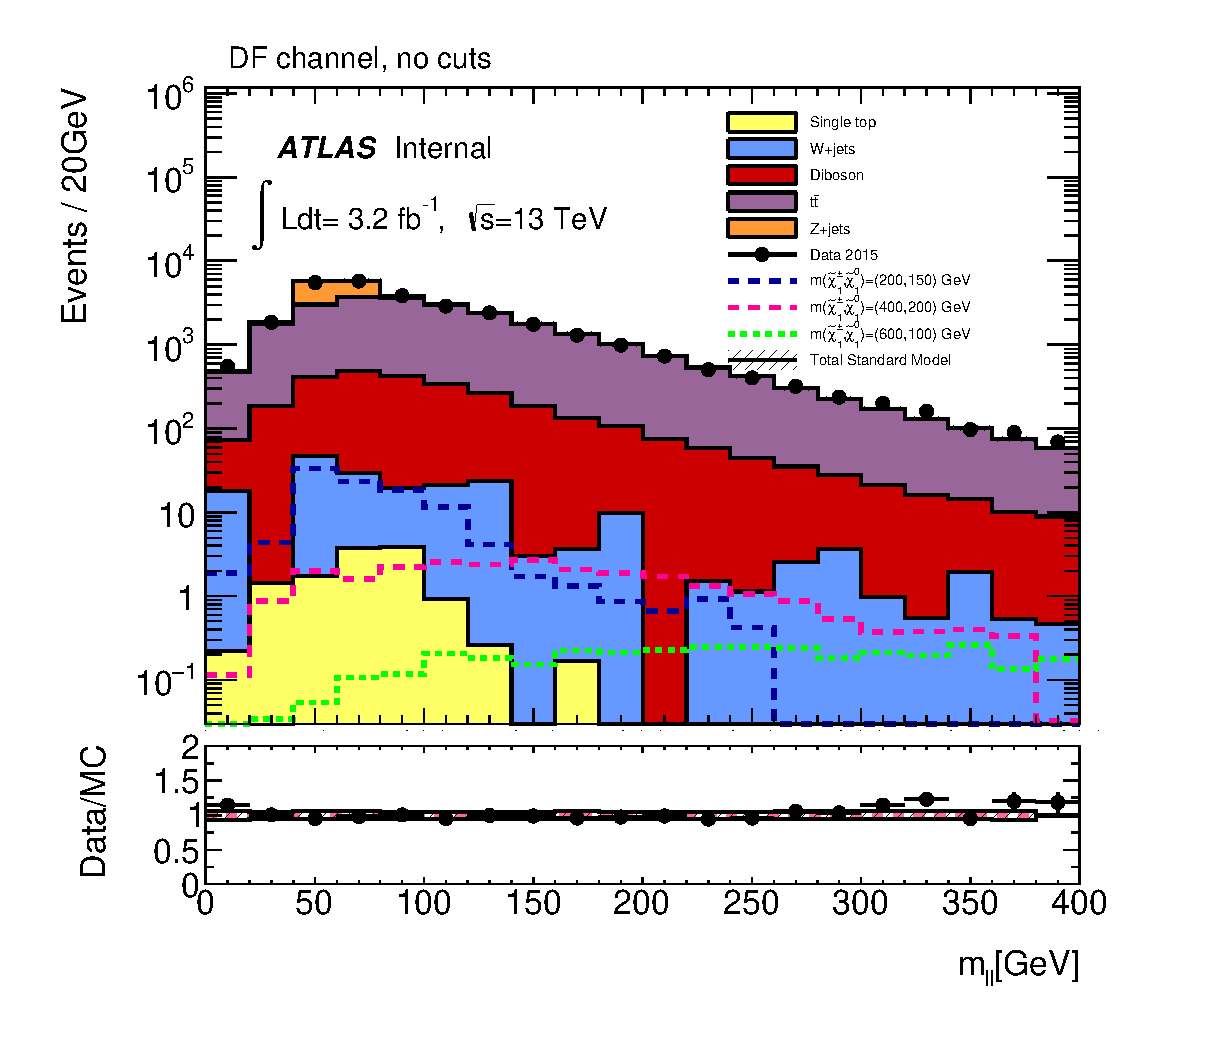
\includegraphics[scale=0.35]{Chap4/Emu_DileptonMll_13TeV_total_signal} 
        \end{subfigure}
\caption{Dilepton invariant mass distributions for SF and DF channels.}	
        \label{fig:Elmu_total_histos}
\end{figure}

The dotted lines are the shapes of signal distributions and they are in accordance with the mass of the chargino pair. The blue line represents 200-150 mass splitting, so its events are concentrated in the lower mass regions. The pink and green lines represent 400-200 and 600-100 signals respectively, and also are distributed according to this logic. 

\section{Cuts in the SF channel}

As was mentioned in the previous section the the following veto was imposed on all the signal regions in SF channel:
\begin{equation*}
|m_{\ell \ell} - m_Z| > 10 \text{ GeV (with } m_Z = 91.2 \text{ GeV}) 
\end{equation*}
The next step was to veto all the jets to reduce $t\bar{t}$ contribution. The result of this combination of vetoes can be seen in Fig. \ref{fig:SF_0jets_mz}. As expected the \mttwo \, distribution is dependent on the mass splitting and is better for 400-200 and 600-100 signals. At this point it is possible to calculate sensitivity values by placing cuts on \mttwo \, and the results can be seen in Tab. \ref{tab:SF_score}. No signal was obtained for 200-150 signal, therefore it is omitted from the table. The best result was the projected significance of 3.62 at 19.2 fb\textsuperscript{-1}  with \mttwo$>100$ GeV cut. 



\begin{figure}[!th]	   
	\begin{subfigure}[t]{0.5\textwidth}
		\subcaption{} 
		\label{fig:SF_0jets_mz_mt2}
        \includegraphics[scale=0.35]{Nojetsmz/SF_DileptonMt2_13TeV_0jets_mz_signal} 
        \end{subfigure} 
     \begin{subfigure}[t]{0.5\textwidth}
     \subcaption{}
     	\label{fig:SF_0jets_mz_metrel}
        \includegraphics[scale=0.35]{Nojetsmz/SF_DileptonMetRel_13TeV_0jets_mz_signal} 
        \end{subfigure}
\caption{The \metrel \, and \mttwo \, distributions for SF channel, with cuts on $m_Z$ and no jets.}	
        \label{fig:SF_0jets_mz}
\end{figure}
\begin{table}[th]
\centering
\begin{tabular}{l|l|l|l|l|l|l|}
\hline
\multicolumn{1}{|l|}{$\int \mathcal{L}\, dt$} & \multicolumn{2}{c|}{3.2 fb\textsuperscript{-1}} & \multicolumn{2}{c|}{9.6 fb\textsuperscript{-1}} & \multicolumn{2}{c|}{19.2 fb\textsuperscript{-1}} \\ \hline
\multicolumn{1}{|l|}{Signal models}               & \textbf{400-200}        & \textbf{600-100}        & \textbf{400-200}        & \textbf{600-100}        & \textbf{400-200}         & \textbf{600-100}        \\ \hline
\multicolumn{1}{|l|}{\mttwo $>80$ GeV}      & 1.01                    & 0.26                    & 1.74                    & 0.45                    & 2.46                     & 0.64                    \\ \hline
\multicolumn{1}{|l|}{\mttwo $>100$ GeV}     & 1.47                    & 0.50                    & 2.56                    & 0.86                    & 3.62                     & 1.22                    \\ \hline
\multicolumn{1}{|l|}{\mttwo $>120$ GeV}     & 1.27                    & 0.61                    & 2.19                    & 1.06                    & 3.09                     & 1.5                     \\ \hline
\end{tabular}
\caption{Significance values ($S/\sqrt{B}$) for the SF channel signal models with various cuts on \mttwo \, at increasing integrated luminosities. For all signals cuts are placed on $m_Z$ and no jets are allowed. }
\label{tab:SF_score}
\end{table}